\Chapter{Aplikacja}\label{chapter:website}

\section{Specyfikacja wymagań}
    \subsection{Wymagania funkcjonalne}\label{subsection:wymagania_funkcjonalne}
        Aplikacja musi realizować cztery kluczowe grupy funkcjonalności:

        \begin{itemize}
            \item \textbf{Obsługa wielu planów i konfiguracji} --- możliwość pracy z wieloma zestawami zasobów i ograniczeń oraz wieloma planami równolegle.
            \item \textbf{Wprowadzanie danych} --- import plików \verb|txt| i \verb|csv| oraz ręczna edycja nauczycieli, klas, przedmiotów, sal, wymagań głównych i bloków przedmiotów
            \item \textbf{Generowanie planu} --- automatyczne tworzenie planów z możliwością kontroli parametrów algorytmu ewolucyjnego
            \item \textbf{Przeglądanie planów} --- wizualizacja planów z perspektywy nauczycieli i klas dla wielu wariantów
        \end{itemize}

    \subsection{Wymagania niefunkcjonalne}
        System musi spełniać następujące wymagania jakościowe:

        \begin{itemize}
            \item \textbf{Wymagania wydajnościowe:}
            \begin{itemize}
                \item Czas generowania kompletnego planu nie powinien przekraczać 10 minut dla typowych przypadków.
                \item Aplikacja musi obsługiwać realistyczne rozmiary danych: do 1000 wymagań głównych, 100 nauczycieli, 50 klas i 100 sal.
                \item Zużycie pamięci operacyjnej nie może przekraczać 8GB podczas generowania planu.
            \end{itemize}
            \item \textbf{Wymagania co do interfejsu:}
            \begin{itemize}
                \item Interfejs powinien być intuicyjny dla użytkowników zaznajomionych z arkuszami kalkulacyjnymi.
                \item Spójność interfejsu we wszystkich modułach aplikacji.
                \item Przejrzystość, minimalizm, wygoda i prostota w użytkowaniu interfejsu.
            \end{itemize}
        \end{itemize}

        Szczegółowa specyfikacja wymagań została przedstawiona na załączonym diagramie przypadków użycia (\ref{fig:diagram_wymagan}).

            \begin{sidewaysfigure}[!p]
                \centering
                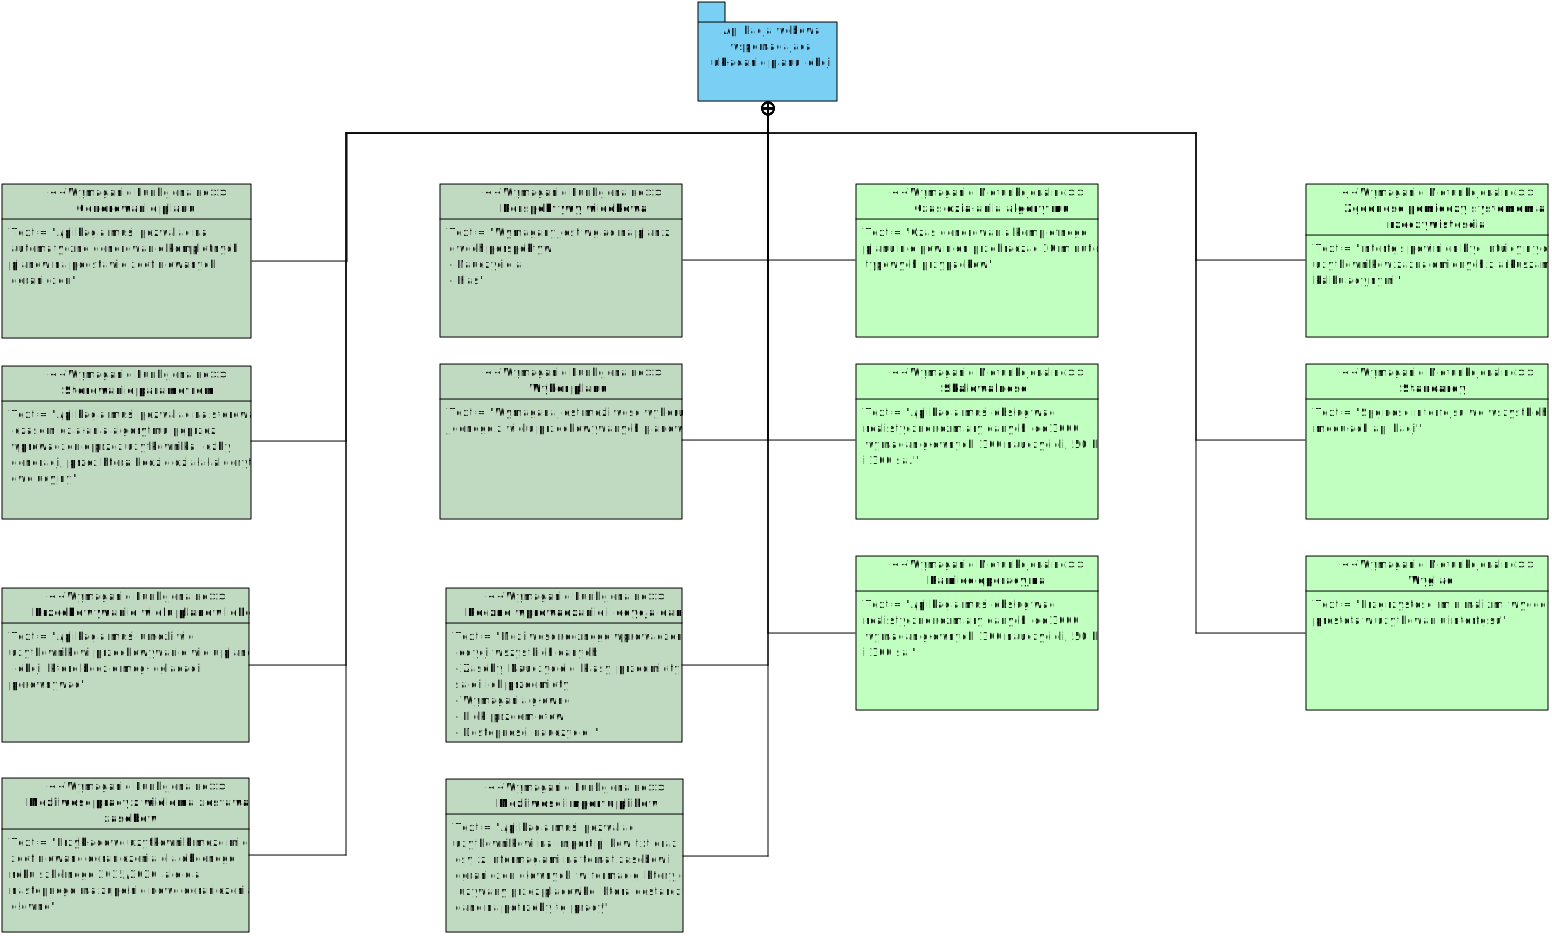
\includegraphics[width=\textwidth,height=\textheight,keepaspectratio]{images/diagramy/Requirement Diagram1.png}
                \caption{Diagram wymagań}\label{fig:diagram_wymagan}
            \end{sidewaysfigure}

    
    % \subsection{Wymagania funkcjonalne}
    %     Najważniejszym aspektem działania aplikacji są funkcjonalności, które ona posiada.
    %     Takie wymagania nazywamy funkcjonalnymi --- definiują one konkretne zachowania i funkcje, które system musi porafić wykonać.

    %     W mojej aplikacji mogę podzielić takie wymagania na 4 grupy:
    %     \begin{itemize}
    %         \item \textbf{Obsługa wielu planów lekcji i konfiguracji:}
    %         \begin{itemize}
    %             \item Tworzenie i przechowywanie wielu planów lekcji.
    %             \item Możliwość pracy z wieloma zestawami zasobów i ograniczeń równolegle.
    %             Przykładowo dla obecnego roku szkolnego mamy zbiór ograniczeń głównych $\mathcal{W}_{2025/2026}$, ale dla następnego jest to juz zupełnie inne zbiór ograniczeń $\mathcal{W}_{2026/2027}$.
    %         \end{itemize}
    %         \item \textbf{Wymagania dotyczące wprowadzania danych:}
    %         \begin{itemize}
    %             \item Import plików \verb|txt| oraz \verb|csv| z zasobami i wymaganiami w formacie używanym przez placówkę, która dostarczyła dane na potrzeby tej pracy.
    %             \item Możliwość ręcznego wprowadzenia i edycji wszystkich typów danych:
    %             \begin{itemize}
    %                 \item Nauczyciele, klasy, przedmioty, sale.
    %                 \item Wymagania główne i bloki przedmiotów.
    %                 \item Dostępności i możliwości sal.
    %             \end{itemize}
    %         \end{itemize}
    %         \item \textbf{Wymagania dotyczące generowania planu lekcji:}
    %         \begin{itemize}
    %             \item Automatyczne generowanie kompletnych planów na podstawie zdefiniowanych ograniczeń.
    %             \item Możliwość sterowania czasem generowania planu poprzez wprowadzanie liczby generacji w algorytmie ewolucyjnym.
    %         \end{itemize}
    %         \item \textbf{Wymagania dotyczące wglądu na utworzone plany:}
    %         \begin{itemize}
    %             \item Wymagany jest wgląd na plan z perspektywy:
    %             \begin{itemize}
    %                 \item Nauczycieli
    %                 \item Klas
    %             \end{itemize}
    %             \item Wymagana jest możliwość wglądu w wiele różnych planów lekcji.
    %         \end{itemize}
    %     \end{itemize}

    % \subsection{Wymagania niefunkcjonalne}
    %     Wymagania niefunkcjonalne określają jakościowe cechy systemu, wpływające na jego użyteczność, wydajność i niezawodność.

    %     Dla rozpatrywanej aplikacji przyjąłem 2 grupy tych wymagań:

    %     \begin{itemize}
    %         \item \textbf{Wymagania wydajnościowe:}
    %         \begin{itemize}
    %             \item Czas generowania kompletnego planu nie powinien przekraczać 10 minut dla typowych przypadków.
    %             \item Aplikacja musi obsługiwać realistyczne rozmiary danych: do 1000 wymagań głównych, 100 nauczycieli, 50 klas i 100 sal.
    %             \item Zużycie pamięci operacyjnej nie może przekraczać 8GB podczas generowania planu.
    %         \end{itemize}
    %         \item \textbf{Wymagania co do interfejsu:}
    %         \begin{itemize}
    %             \item Interfejs powinien być intuicyjny dla użytkowników zaznajomionych z arkuszami kalkulacyjnymi.
    %             \item Spójność interfejsu we wszystkich modułach aplikacji.
    %             \item Przejrzystość, minimalizm, wygoda i prostota w użytkowaniu interfejsu.
    %         \end{itemize}
    %     \end{itemize}

    %     Uwzględnienie zarówno wymagań funkcjonalnych, jak i niefunkcjonalnych pozwala na stworzenie kompletnej aplikacji, która nie tylko realizuje założone funkcje, ale także zapewnia komfortowe i niezawodne środowisko pracy dla docelowych użytkowników.

    \subsection{Przypadki użycia}
        Diagram przypadków użycia pozwala na zwizualizowanie wcześniej omawianych wymagań funkcjonalnych w formie graficznej, ukazując interakcje między użytkownikami a systemem.
        Diagram służy jako most pomiędzy specyfikacją wymagań a projektem technicznym, stanowiąc punkt wyjścia do dalszej analizy i implementacji.
        W niniejszej sekcji omawiam kluczowe przypadki użycia zilustrowane na diagramie.

        \begin{figure}[!h]
            \centering
            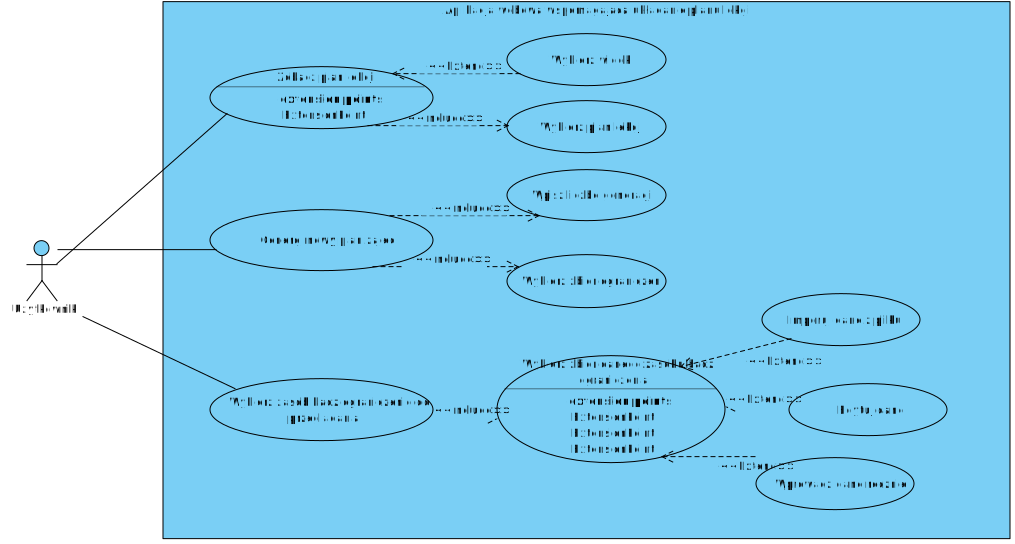
\includegraphics[width=1.0\textwidth]{images/diagramy/Use Case Diagram1.png}
            \caption{Diagram przypadków użycia}\label{fig:usecases}
        \end{figure}

        \textit{Opis w tabelach}

    \subsection{Diagramy sekwencji}
        Diagramy sekwencji stanowią kluczowy element modelowania systemu, ukazując sekwencyjny przepływ komunikatów między obiektami w czasie.
        Pozwalają prześledzić pełny cykl życia żądań użytkownika --- od inicjacji akcji w interfejsie, poprzez przetwarzanie w backendzie, aż do generowania planu przez specjalistyczne algorytmy.
        W niniejszej sekcji przedstawiam scenariusze współpracy pomiędzy głównymi komponentami aplikacji: interfejsem, warstwą serwerową oraz algorytmem.

        \begin{figure}[!t]
            \centering
            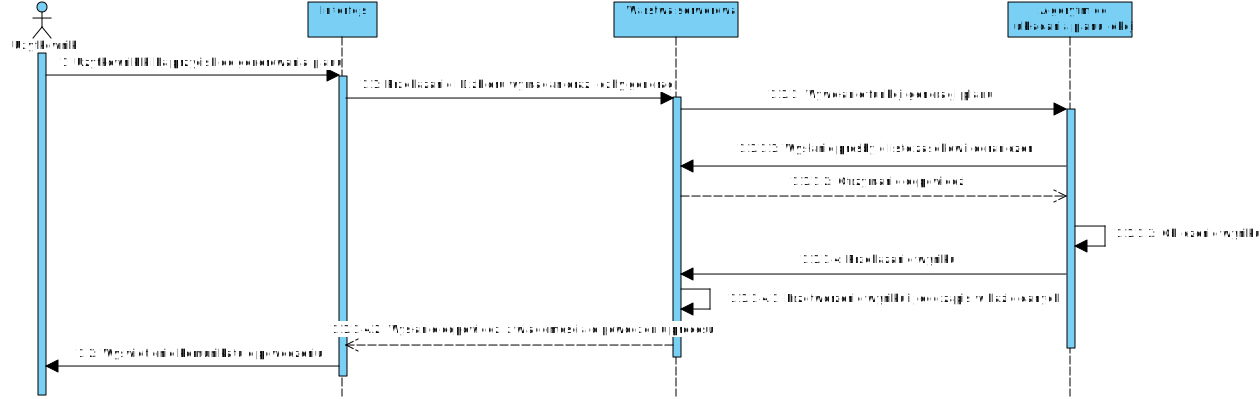
\includegraphics[width=1.0\textwidth]{images/diagramy/Sequence Diagram1.png}
            \caption{Diagram sekwencji dla przypadku użycia generowania planu lekcji}
        \end{figure}
        
        \begin{figure}[!t]
            \centering
            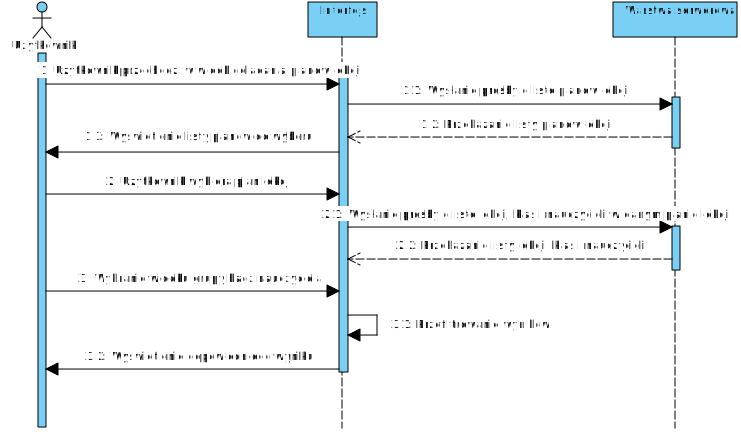
\includegraphics[width=1.0\textwidth]{images/diagramy/Sequence Diagram2.png}
            \caption{Diagram sekwencji dla przypadku użycia oglądania planu lekcji}
        \end{figure}

        \begin{figure}[!t]
            \centering
            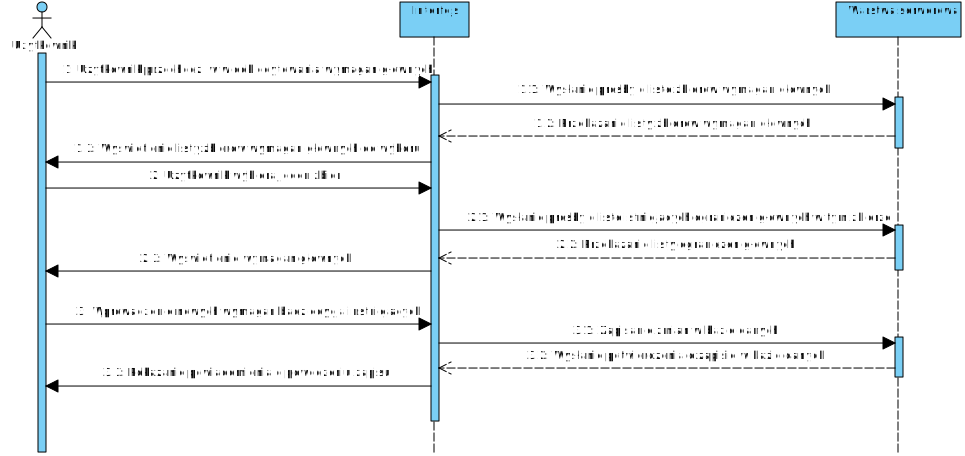
\includegraphics[width=1.0\textwidth]{images/diagramy/Sequence Diagram3.png}
            \caption{Diagram sekwencji dla przypadku użycia edycji bądź wprowadzania wymagań głównych}
        \end{figure}

        \FloatBarrier

\newpage
\section{Projekt}
    \subsection{Projekt struktury bazy danych}
        Projekt bazy danych stanowi kluczowy element architektury aplikacji webowej, determinujący jej skalowalność i funkcjonalność. 
        Głównym wyzwaniem projektowym było opracowanie modelu umożliwiającego wielokrotne wykorzystanie tych samych zasobów przy jednoczesnej obsłudze zmieniających się wymagań głównych pomiędzy generowaniami planów lekcji. 
        W odpowiedzi na to wymaganie wprowadziłem mechanizm grupowania zasobów i ograniczeń w zbiory, co zapewnia elastyczność niezbędną w środowisku szkolnym.
        W celu wyjaśnienia tej skomplikowanej struktury bazy danych warto podzielić tabele na parę kategorii.

        \subsubsection{Tabele podstawowe}
            Tabele podstawowe definiują fundamentalne zasoby szkoły, stanowiąc punkt odniesienia dla całego systemu:
            \begin{table}[H]
                \centering
                \begin{tabular}{|r|l|}
                    \hline
                    \textbf{Tabela} & \textbf{Relacja} \\
                    \hline
                    \texttt{subject} & \\
                    \texttt{student\_group} & \\
                    \texttt{teacher} & M:N do \texttt{subject} \\
                    \texttt{room} & M:N do \texttt{subject} \\
                    \hline
                \end{tabular}
                \caption{Tabele podstawowe zasobów szkolnych}
            \end{table}

            \noindent
            gdzie:
            \begin{itemize}
                \item \texttt{subject} przychowuje przedmioty.
                \item \texttt{student\_group} przechowuje przedmioty.
                \item \texttt{teacher} przechowuje nauczycieli.
                \item \texttt{room} przechowuje sale.
            \end{itemize}

            Relacja między nauczycielami a przedmiotami reprezentuje prowadzone przez nich przedmioty, a relacja między salami a przedmiotami reprezentuje przedmioty, które są przez nie obsługiwane.

            \begin{figure}[H]
                \centering
                \includegraphics[width=0.5\textwidth]{images/diagramy/diagram_db_podstawowe.png}
                \caption{Diagram tabel podstawowych w bazie danych}
            \end{figure}

        \subsubsection{Tabele wymagań}
            Tabele wymagań przechowują ograniczenia i reguły generowania planu, powiązane z zasobami podstawowymi:

            \begin{table}[H]
                \centering
                \begin{tabular}{|r|l|}
                    \hline
                    \textbf{Tabela} & \textbf{Relacje} \\
                    \hline
                    \texttt{requirement} & N:1 z \texttt{teacher}, \texttt{student\_group}, \texttt{subject} \\
                    \texttt{subject\_block} & M:N z \texttt{subject} \\
                    \texttt{teacher\_availability} & N:1 z \texttt{teacher} \\
                    \hline
                \end{tabular}
                \caption{Tabele definiujące wymagania i ograniczenia}
            \end{table}

            \noindent
            gdzie:
            \begin{itemize}
                \item \texttt{requirement} przychowuje wymagania główne.
                \item \texttt{subject\_block} przechowuje informacje na temat bloków przedmiotów.
                \item \texttt{teacher\_availability} przechowuje dostępności nauczycieli.
            \end{itemize}

            \begin{figure}[H]
                \centering
                \includegraphics[width=0.8\textwidth]{images/diagramy/diagram_db_wymagan.png}
                \caption{Diagram tabel podstawowych i wymagań w bazie danych}
            \end{figure}

        \subsubsection{Tabele agregujące}
            Mechanizm zbiorów umożliwia grupowanie zasobów i wymagań dla różnych kontekstów:

            \begin{table}[H]
                \centering
                \begin{tabular}{|r|l|}
                    \hline
                    \textbf{Tabela} & \textbf{Relacja} \\
                    \hline
                    \texttt{subject\_pool} & M:N z subject \\
                    \texttt{student\_group\_pool} & 1:N z student\_group \\
                    \texttt{teacher\_pool} & M:N z teacher \\
                    \texttt{room\_pool} & 1:N z room \\
                    \hline
                \end{tabular}
                \caption{Tabele zbiorów zasobów z uzasadnieniem relacji}
            \end{table}

            Dla nauczycieli i przedmiotów zastosowałem relację wiele-do-wielu, ponieważ zasoby te charakteryzują się względną stabilnością pomiędzy latami szkolnymi --- większość nauczycieli i przedmiotów pozostaje niezmieniona, a jedynie dodawane są nowe rekordy dla nowo zatrudnionych pedagogów lub wprowadzanych przedmiotów.
            
            W przypadku sal przyjęto relację jeden-do-wielu, co wynika z całkowitej niezmienności tej puli zasobów pomiędzy okresami szkolnymi.
            Natomiast dla klas zastosowałem relację jeden-do-wielu, odzwierciedlającą coroczną całkowitą wymianę składu grup uczniowskich --- klasy z poprzedniego roku nie są ponownie wykorzystywane w kolejnych okresach, co eliminuje potrzebę stosowania relacji wiele-do-wielu.

            Szczególną rolę pełni tabela \texttt{requirement\_set} (zbiór wymagań głównych), która agreguje wszystkie wymagania poprzez relacje 1:N z \texttt{requirement}, \texttt{teacher\_availability}, \texttt{subject\_block} oraz relacje N:1 z pozostałymi zbiorami.
            Ta struktura umożliwia generowanie kompletnego planu lekcji na podstawie pojedynczego rekordu zbioru wymagań.
            % \begin{enumerate}
            %     \item[5.] Tabela zbiorów \textbf{wymagań głównych} \verb|req_set|.
            %     \begin{itemize}
            %         \item Relacja jeden do wielu z tabelą wymagań głównych
            %         \item Relacja jeden do wielu z tabelą dostępności nauczycieli
            %         \item Relacja jeden do wielu z tabelą bloków przedmiotów
            %         \item Relacja wiele do jeden z tabelą zbiorów klas, nauczycieli oraz sal
            %     \end{itemize}
            % \end{enumerate}

            Zaprezentowany model bazy danych zapewnia elastyczność niezbędną do obsługi zmieniających się wymagań szkolnych poprzez mechanizm zbiorów. Struktura umożliwia wielokrotne wykorzystanie zasobów pomiędzy różnymi konfiguracjami planów, zachowując przy tym prostotę i wydajność.

        \subsubsection{Tabele wyników}
            Tabele przechowujące wygenerowane plany lekcji i ich przypisania:

            \begin{table}[H]
                \centering
                \begin{tabular}{|l|l|}
                    \hline
                    \textbf{Tabela} & \textbf{Relacje} \\
                    \hline
                    \texttt{plan} & N:1 z requirement\_set \\
                    \texttt{lesson} & N:1 z teacher, subject, room, student\_group, plan \\
                    \hline
                \end{tabular}
                \caption{Tabele przechowujące wygenerowane plany lekcji}
            \end{table}

            \noindent
            gdzie:
            \begin{itemize}
                \item \texttt{plan} przychowuje plany lekcji.
                \item \texttt{lesson} przechowuje przypisania.
            \end{itemize}

        \begin{figure}[p]
            \centering
            \includegraphics[width=1.0\textwidth]{images/diagramy/diagram_db.png}
            \caption{Diagram pełnego projektu bazy danych}
        \end{figure}

        \begin{table}[p]
            \centering
            \begin{tabular}{|p{0.27\textwidth}|p{0.2\textwidth}|p{0.45\textwidth}|}
                \hline
                \textbf{Tabela} & \textbf{Kolumna} & \textbf{Opis} \\
                \hline
                \multirow{3}{*}{\texttt{student\_group}} & \texttt{id} & Unikalny identyfikator klasy \\
                & \texttt{pool\_id} & Klucz obcy do zbioru klas \\
                & \texttt{name} & Nazwa klasy (,,IIIA'') \\
                & \texttt{desc} & Opis klasy (opcjonalny) \\
                \hline
                \multirow{3}{*}{\texttt{room}} & \texttt{id} & Unikalny identyfikator sali \\
                & \texttt{pool\_id} & Klucz obcy do zbioru sal \\
                & \texttt{name} & Nazwa sali (,,Sala 101'') \\
                \hline
                \multirow{1}{*}{\texttt{subject}} & \texttt{id} & Unikalny identyfikator przedmiotu \\
                & \texttt{name} & Nazwa przedmiotu (,,Matematyka'') \\
                \hline
                \multirow{2}{*}{\texttt{teacher}} & \texttt{id} & Unikalny identyfikator nauczyciela \\
                & \texttt{name} & Imię i/lub nazwisko nauczyciela \\
                \hline
                \multirow{6}{*}{\texttt{requirement\_set}} & \texttt{id} & Unikalny identyfikator zbioru wymagań \\
                & \texttt{teacher\_pool\_id} & Klucz obcy do zbioru nauczycieli \\
                & \texttt{room\_pool\_id} & Klucz obcy do zbioru sal \\
                & \texttt{group\_pool\_id} & Klucz obcy do zbioru klas \\
                & \texttt{subject\_pool\_id} & Klucz obcy do zbioru przedmiotów \\
                & \texttt{name} & Nazwa zbioru wymagań \\
                \hline
                \multirow{4}{*}{\texttt{subject\_block}} & \texttt{id} & Unikalny identyfikator bloku przedmiotów \\
                & \texttt{req\_set\_id} & Klucz obcy do zbioru wymagań \\
                & \texttt{numbers} & Konfiguracja liczby godzin (JSON) \\
                & \texttt{power\_block} & Flaga bloku agregującego \\
                & \texttt{max\_number} & Maksymalna liczba bloków tygodniowo \\
                \hline
                \multirow{3}{*}{\texttt{requirement}} & \texttt{id} & Unikalny identyfikator wymagania \\
                & \texttt{req\_set\_id} & Klucz obcy do zbioru wymagań \\
                & \texttt{teacher\_id} & Klucz obcy do nauczyciela \\
                & \texttt{group\_id} & Klucz obcy do klasy \\
                & \texttt{subject\_id} & Klucz obcy do przedmiotu \\
                & \texttt{hours} & Liczba wymaganych godzin tygodniowo \\
                \hline
                \multirow{3}{*}{\texttt{teacher\_availability}} & \texttt{id} & Unikalny identyfikator dostępności \\
                & \texttt{teacher\_id} & Klucz obcy do nauczyciela \\
                & \texttt{req\_set\_id} & Klucz obcy do zbioru wymagań \\
                & \texttt{availability} & Macierz dostępności (JSON) \\
                \hline
                \multirow{3}{*}{\texttt{plan}} & \texttt{id} & Unikalny identyfikator planu \\
                & \texttt{req\_set\_id} & Klucz obcy do zbioru wymagań \\
                & \texttt{name} & Nazwa planu lekcji \\
                \hline
                \multirow{7}{*}{\texttt{lesson}} & \texttt{id} & Unikalny identyfikator lekcji \\
                & \texttt{plan\_id} & Klucz obcy do planu \\
                & \texttt{teacher\_id} & Klucz obcy do nauczyciela \\
                & \texttt{subject\_id} & Klucz obcy do przedmiotu \\
                & \texttt{room\_id} & Klucz obcy do sali \\
                & \texttt{student\_group\_id} & Klucz obcy do klasy \\
                & \texttt{day} & Dzień tygodnia \\
                & \texttt{hour} & Slot czasowy \\
                \hline
            \end{tabular}
            \caption{Struktura wszystkich tabel}
        \end{table}
    \clearpage

    \subsection{Projekt interfejsu}
        abc

    \subsection{Sposób integracji z algorytmem}
        abc
        
\section{Implementacja}
    \subsection{Wybór narzędzi}
        Dlaczego React+Django. Dlaczego PostgreSQL
    \subsection{Implementacja bazy danych w Django}
    \subsection{Implementacja API w Django}
    \subsection{Implementacja interfejsu w React}
    \subsection{Integracja z algorytmem}